\documentclass[9pt,twocolumn,twoside]{osajnl}
\usepackage{xeCJK}
\usepackage{indentfirst}
\journal{ol} % Choose journal (ao, aop, josaa, josab, ol)

% See template introduction for guidance on setting shortarticle option
\setboolean{shortarticle}{false} 
% true = letter / tutorial 
% false = research / review article 
% (depending on journal).


\title{基于多人三维五子棋对弈的蒙特卡洛树搜索算法}

\author[1]{吴佳成}

\affil[1]{南开大学,软件学院,软件工程专业,三班,1412649}

%% To be edited by editor
\dates{\today}

\begin{abstract}

\ \ \ \ \ 基于蒙特卡洛树搜索来解决对弈问题的想法早已有之,然而蒙特卡洛树搜索算法在多人对弈中的研究并不常见。一方面,多人对弈中的情况较为复杂,多方之间的关系并不仅仅是单纯的对抗关系,另外一方面,数的搜索也会随着人数的增加而造成更为复杂的情况。本文用一些相对较为简单的五子棋为例来进行多人对弈的蒙特卡洛树搜索。
\newline
\newline
关键字:多人对弈、蒙特卡洛树搜索
\end{abstract}

\begin{document}

\maketitle

\section{引言}

This template is designed to assist with creating an article to submit to \emph{Applied Optics}, \emph{Advances in Optics and Photonics}, JOSA A, JOSA B, or \emph{Optics Letters}. See the OSA's \href{http://www.opticsinfobase.org/submit/style/}{Style Guide} and \href{http://www.opticsinfobase.org/submit/templates/}{Manuscript Templates} pages for more details. Please select the appropriate journal abbreviation (ao, aop, josaa, josab, ol) in the document preamble.

Use the shortarticle/false option for \emph{Applied Optics}, JOSA A, and JOSA B. Use the shortarticle/true option for \emph{Optics Letters}. For \emph{Advances in Optics and Photonics}, use the shortarticle/false option for Review Articles, and the shortarticle/true option for Tutorials.

If you have a question while using this template on {Overleaf}, please use the help menu (``?'') on the top bar to search for help or ask us a question using our \href{https://www.overleaf.com/contact}{contact form}.

\section{Examples of Article Components}
\label{sec:examples}

The sections below show examples of different article components.

\section{Figures and Tables}

It is not necessary to place figures and tables at the back of the manuscript. Figures and tables should be sized as they are to appear in the final article. Do not include a separate list of figure captions and table titles.

Figures and Tables should be labelled and referenced in the standard way using the \verb|\label{}| and \verb|\ref{}| commands.

\subsection{Sample Figure}

Figure \ref{fig:false-color} shows an example figure.

\begin{figure}[htbp]
\centering
\fbox{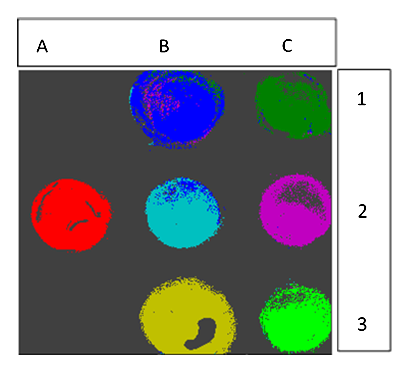
\includegraphics[width=\linewidth]{sample}}
\caption{False-color image, where each pixel is assigned to one of seven reference spectra.}
\label{fig:false-color}
\end{figure}

\subsection{Sample Table}

Table \ref{tab:shape-functions} shows an example table.

\begin{table}[htbp]
\centering
\caption{\bf Shape Functions for Quadratic Line Elements}
\begin{tabular}{ccc}
\hline
local node & $\{N\}_m$ & $\{\Phi_i\}_m$ $(i=x,y,z)$ \\
\hline
$m = 1$ & $L_1(2L_1-1)$ & $\Phi_{i1}$ \\
$m = 2$ & $L_2(2L_2-1)$ & $\Phi_{i2}$ \\
$m = 3$ & $L_3=4L_1L_2$ & $\Phi_{i3}$ \\
\hline
\end{tabular}
  \label{tab:shape-functions}
\end{table}

\section{Sample Equation}

Let $X_1, X_2, \ldots, X_n$ be a sequence of independent and identically distributed random variables with $\text{E}[X_i] = \mu$ and $\text{Var}[X_i] = \sigma^2 < \infty$, and let
\begin{equation}
S_n = \frac{X_1 + X_2 + \cdots + X_n}{n}
      = \frac{1}{n}\sum_{i}^{n} X_i
\label{eq:refname1}
\end{equation}
denote their mean. Then as $n$ approaches infinity, the random variables $\sqrt{n}(S_n - \mu)$ converge in distribution to a normal $\mathcal{N}(0, \sigma^2)$.

\section{Sample Algorithm}

Algorithms can be included using the commands as shown in algorithm \ref{alg:euclid}.

\begin{algorithm}
\caption{Euclid’s algorithm}\label{alg:euclid}
\begin{algorithmic}[1]
\Procedure{Euclid}{$a,b$}\Comment{The g.c.d. of a and b}
\State $r\gets a\bmod b$
\While{$r\not=0$}\Comment{We have the answer if r is 0}
\State $a\gets b$
\State $b\gets r$
\State $r\gets a\bmod b$
\EndWhile\label{euclidendwhile}
\State \textbf{return} $b$\Comment{The gcd is b}
\EndProcedure
\end{algorithmic}
\end{algorithm}

\section{Supplemental Material}

Consult the Author Guidelines for Supplementary Materials in OSA Journals for details on accepted types of materials and instructions on how to cite them.
All materials must be associated with a figure, table, or equation or be referenced in the results section of the manuscript. 
(1) 2D and 3D image files and video must be labeled “Visualization,” not “Movie,” “Video,” “Figure,” etc. 
(2) Machine-readable data (for example, csv files) must be labeled  “Data File.”  Number data files and visualizations consecutively, e.g., “Visualization 1, Visualization 2….”
(3) Large datasets or code files must be placed in an open, archival database.  Such items should be mentioned in the text as either “Dataset” or “Code,” as appropriate, and also be cited in the references list.  For example, “see Dataset 1 (Ref. [1]) and Code 1 (Ref [2]).” Here are examples of the references: 


\subsection{Sample Code Citation}

2. C. Rivers, "Epipy: Python tools for epidemiology" (Figshare, 2014) [retrieved 13 May 2015], http://dx.doi.org/10.6084/m9.figshare.1005064.



%Manual citation list
\begin{thebibliography}{1}
\bibitem{Zhang:14}
Y.~Zhang, S.~Qiao, L.~Sun, Q.~W. Shi, W.~Huang, L.~Li, and Z.~Yang, \emph{Photoinduced active terahertz metamaterials with nanostructured vanadium dioxide film deposited by sol-gel method,} Opt. Express \textbf{22}, 11070--11078 (2014).
\bibitem{test} .
\end{thebibliography}


\end{document}
